%--------------------------------------------------------------------------
%
%                                                    ENONCE
%
%--------------------------------------------------------------------------
%test
\begin{center}
\vspace*{5mm}
\noindent {\Large {\bf (Problem) }}
\end{center}

\begin{enumerate}
\item[a)] The numbered squares in the figure below represent the position of two blocs at 0.20 s intervals. The blocs are moving in the left to right direction. Compare their acceleration.
\begin{center}
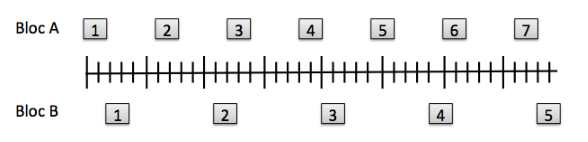
\includegraphics{figures/serie01_concept1.pdf}
\end{center}

\item[b)] A spaceship drifts sideways in space between point P and Q. It is not subject to any external force. At point Q, the spaceship's engine is turned on and produces a constant acceleration perpendicular to PQ. This acceleration is maintained until the spaceship reaches a point R. Which of the following trajectories best represents the ship's path?

\begin{center}
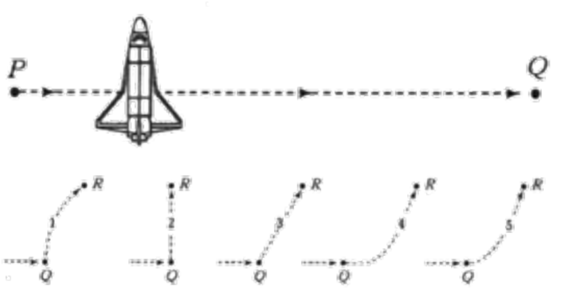
\includegraphics{figures/serie01_concept2.pdf}
\end{center}
\end{enumerate}
